\documentclass[]{book}
\usepackage{lmodern}
\usepackage{amssymb,amsmath}
\usepackage{ifxetex,ifluatex}
\usepackage{fixltx2e} % provides \textsubscript
\ifnum 0\ifxetex 1\fi\ifluatex 1\fi=0 % if pdftex
  \usepackage[T1]{fontenc}
  \usepackage[utf8]{inputenc}
\else % if luatex or xelatex
  \ifxetex
    \usepackage{mathspec}
  \else
    \usepackage{fontspec}
  \fi
  \defaultfontfeatures{Ligatures=TeX,Scale=MatchLowercase}
\fi
% use upquote if available, for straight quotes in verbatim environments
\IfFileExists{upquote.sty}{\usepackage{upquote}}{}
% use microtype if available
\IfFileExists{microtype.sty}{%
\usepackage{microtype}
\UseMicrotypeSet[protrusion]{basicmath} % disable protrusion for tt fonts
}{}
\usepackage[margin=1in]{geometry}
\usepackage{hyperref}
\hypersetup{unicode=true,
            pdftitle={Orchestrating Single-Cell Analysis},
            pdfauthor={Bioconductor},
            pdfborder={0 0 0},
            breaklinks=true}
\urlstyle{same}  % don't use monospace font for urls
\usepackage{natbib}
\bibliographystyle{apalike}
\usepackage{color}
\usepackage{fancyvrb}
\newcommand{\VerbBar}{|}
\newcommand{\VERB}{\Verb[commandchars=\\\{\}]}
\DefineVerbatimEnvironment{Highlighting}{Verbatim}{commandchars=\\\{\}}
% Add ',fontsize=\small' for more characters per line
\usepackage{framed}
\definecolor{shadecolor}{RGB}{248,248,248}
\newenvironment{Shaded}{\begin{snugshade}}{\end{snugshade}}
\newcommand{\AlertTok}[1]{\textcolor[rgb]{0.94,0.16,0.16}{#1}}
\newcommand{\AnnotationTok}[1]{\textcolor[rgb]{0.56,0.35,0.01}{\textbf{\textit{#1}}}}
\newcommand{\AttributeTok}[1]{\textcolor[rgb]{0.77,0.63,0.00}{#1}}
\newcommand{\BaseNTok}[1]{\textcolor[rgb]{0.00,0.00,0.81}{#1}}
\newcommand{\BuiltInTok}[1]{#1}
\newcommand{\CharTok}[1]{\textcolor[rgb]{0.31,0.60,0.02}{#1}}
\newcommand{\CommentTok}[1]{\textcolor[rgb]{0.56,0.35,0.01}{\textit{#1}}}
\newcommand{\CommentVarTok}[1]{\textcolor[rgb]{0.56,0.35,0.01}{\textbf{\textit{#1}}}}
\newcommand{\ConstantTok}[1]{\textcolor[rgb]{0.00,0.00,0.00}{#1}}
\newcommand{\ControlFlowTok}[1]{\textcolor[rgb]{0.13,0.29,0.53}{\textbf{#1}}}
\newcommand{\DataTypeTok}[1]{\textcolor[rgb]{0.13,0.29,0.53}{#1}}
\newcommand{\DecValTok}[1]{\textcolor[rgb]{0.00,0.00,0.81}{#1}}
\newcommand{\DocumentationTok}[1]{\textcolor[rgb]{0.56,0.35,0.01}{\textbf{\textit{#1}}}}
\newcommand{\ErrorTok}[1]{\textcolor[rgb]{0.64,0.00,0.00}{\textbf{#1}}}
\newcommand{\ExtensionTok}[1]{#1}
\newcommand{\FloatTok}[1]{\textcolor[rgb]{0.00,0.00,0.81}{#1}}
\newcommand{\FunctionTok}[1]{\textcolor[rgb]{0.00,0.00,0.00}{#1}}
\newcommand{\ImportTok}[1]{#1}
\newcommand{\InformationTok}[1]{\textcolor[rgb]{0.56,0.35,0.01}{\textbf{\textit{#1}}}}
\newcommand{\KeywordTok}[1]{\textcolor[rgb]{0.13,0.29,0.53}{\textbf{#1}}}
\newcommand{\NormalTok}[1]{#1}
\newcommand{\OperatorTok}[1]{\textcolor[rgb]{0.81,0.36,0.00}{\textbf{#1}}}
\newcommand{\OtherTok}[1]{\textcolor[rgb]{0.56,0.35,0.01}{#1}}
\newcommand{\PreprocessorTok}[1]{\textcolor[rgb]{0.56,0.35,0.01}{\textit{#1}}}
\newcommand{\RegionMarkerTok}[1]{#1}
\newcommand{\SpecialCharTok}[1]{\textcolor[rgb]{0.00,0.00,0.00}{#1}}
\newcommand{\SpecialStringTok}[1]{\textcolor[rgb]{0.31,0.60,0.02}{#1}}
\newcommand{\StringTok}[1]{\textcolor[rgb]{0.31,0.60,0.02}{#1}}
\newcommand{\VariableTok}[1]{\textcolor[rgb]{0.00,0.00,0.00}{#1}}
\newcommand{\VerbatimStringTok}[1]{\textcolor[rgb]{0.31,0.60,0.02}{#1}}
\newcommand{\WarningTok}[1]{\textcolor[rgb]{0.56,0.35,0.01}{\textbf{\textit{#1}}}}
\usepackage{longtable,booktabs}
\usepackage{graphicx,grffile}
\makeatletter
\def\maxwidth{\ifdim\Gin@nat@width>\linewidth\linewidth\else\Gin@nat@width\fi}
\def\maxheight{\ifdim\Gin@nat@height>\textheight\textheight\else\Gin@nat@height\fi}
\makeatother
% Scale images if necessary, so that they will not overflow the page
% margins by default, and it is still possible to overwrite the defaults
% using explicit options in \includegraphics[width, height, ...]{}
\setkeys{Gin}{width=\maxwidth,height=\maxheight,keepaspectratio}
\IfFileExists{parskip.sty}{%
\usepackage{parskip}
}{% else
\setlength{\parindent}{0pt}
\setlength{\parskip}{6pt plus 2pt minus 1pt}
}
\setlength{\emergencystretch}{3em}  % prevent overfull lines
\providecommand{\tightlist}{%
  \setlength{\itemsep}{0pt}\setlength{\parskip}{0pt}}
\setcounter{secnumdepth}{5}
% Redefines (sub)paragraphs to behave more like sections
\ifx\paragraph\undefined\else
\let\oldparagraph\paragraph
\renewcommand{\paragraph}[1]{\oldparagraph{#1}\mbox{}}
\fi
\ifx\subparagraph\undefined\else
\let\oldsubparagraph\subparagraph
\renewcommand{\subparagraph}[1]{\oldsubparagraph{#1}\mbox{}}
\fi

%%% Use protect on footnotes to avoid problems with footnotes in titles
\let\rmarkdownfootnote\footnote%
\def\footnote{\protect\rmarkdownfootnote}

%%% Change title format to be more compact
\usepackage{titling}

% Create subtitle command for use in maketitle
\newcommand{\subtitle}[1]{
  \posttitle{
    \begin{center}\large#1\end{center}
    }
}

\setlength{\droptitle}{-2em}

  \title{Orchestrating Single-Cell Analysis}
    \pretitle{\vspace{\droptitle}\centering\huge}
  \posttitle{\par}
    \author{Bioconductor}
    \preauthor{\centering\large\emph}
  \postauthor{\par}
      \predate{\centering\large\emph}
  \postdate{\par}
    \date{2019-01-07}

\usepackage{booktabs}

\begin{document}
\maketitle

{
\setcounter{tocdepth}{1}
\tableofcontents
}
\hypertarget{prerequisites}{%
\chapter{Prerequisites}\label{prerequisites}}

This is a \emph{sample} book written in \textbf{Markdown}. You can use anything that Pandoc's Markdown supports, e.g., a math equation \(a^2 + b^2 = c^2\).

The \textbf{bookdown} package can be installed from CRAN or Github:

\begin{Shaded}
\begin{Highlighting}[]
\KeywordTok{install.packages}\NormalTok{(}\StringTok{"bookdown"}\NormalTok{)}
\CommentTok{# or the development version}
\CommentTok{# devtools::install_github("rstudio/bookdown")}
\end{Highlighting}
\end{Shaded}

Remember each Rmd file contains one and only one chapter, and a chapter is defined by the first-level heading \texttt{\#}.

To compile this example to PDF, you need XeLaTeX. You are recommended to install TinyTeX (which includes XeLaTeX): \url{https://yihui.name/tinytex/}.

\hypertarget{intro}{%
\chapter{Introduction}\label{intro}}

You can label chapter and section titles using \texttt{\{\#label\}} after them, e.g., we can reference Chapter \ref{intro}. If you do not manually label them, there will be automatic labels anyway, e.g., Chapter \ref{methods}.

Figures and tables with captions will be placed in \texttt{figure} and \texttt{table} environments, respectively.

\begin{Shaded}
\begin{Highlighting}[]
\KeywordTok{par}\NormalTok{(}\DataTypeTok{mar =} \KeywordTok{c}\NormalTok{(}\DecValTok{4}\NormalTok{, }\DecValTok{4}\NormalTok{, }\FloatTok{.1}\NormalTok{, }\FloatTok{.1}\NormalTok{))}
\KeywordTok{plot}\NormalTok{(pressure, }\DataTypeTok{type =} \StringTok{'b'}\NormalTok{, }\DataTypeTok{pch =} \DecValTok{19}\NormalTok{)}
\end{Highlighting}
\end{Shaded}

\begin{figure}

{\centering 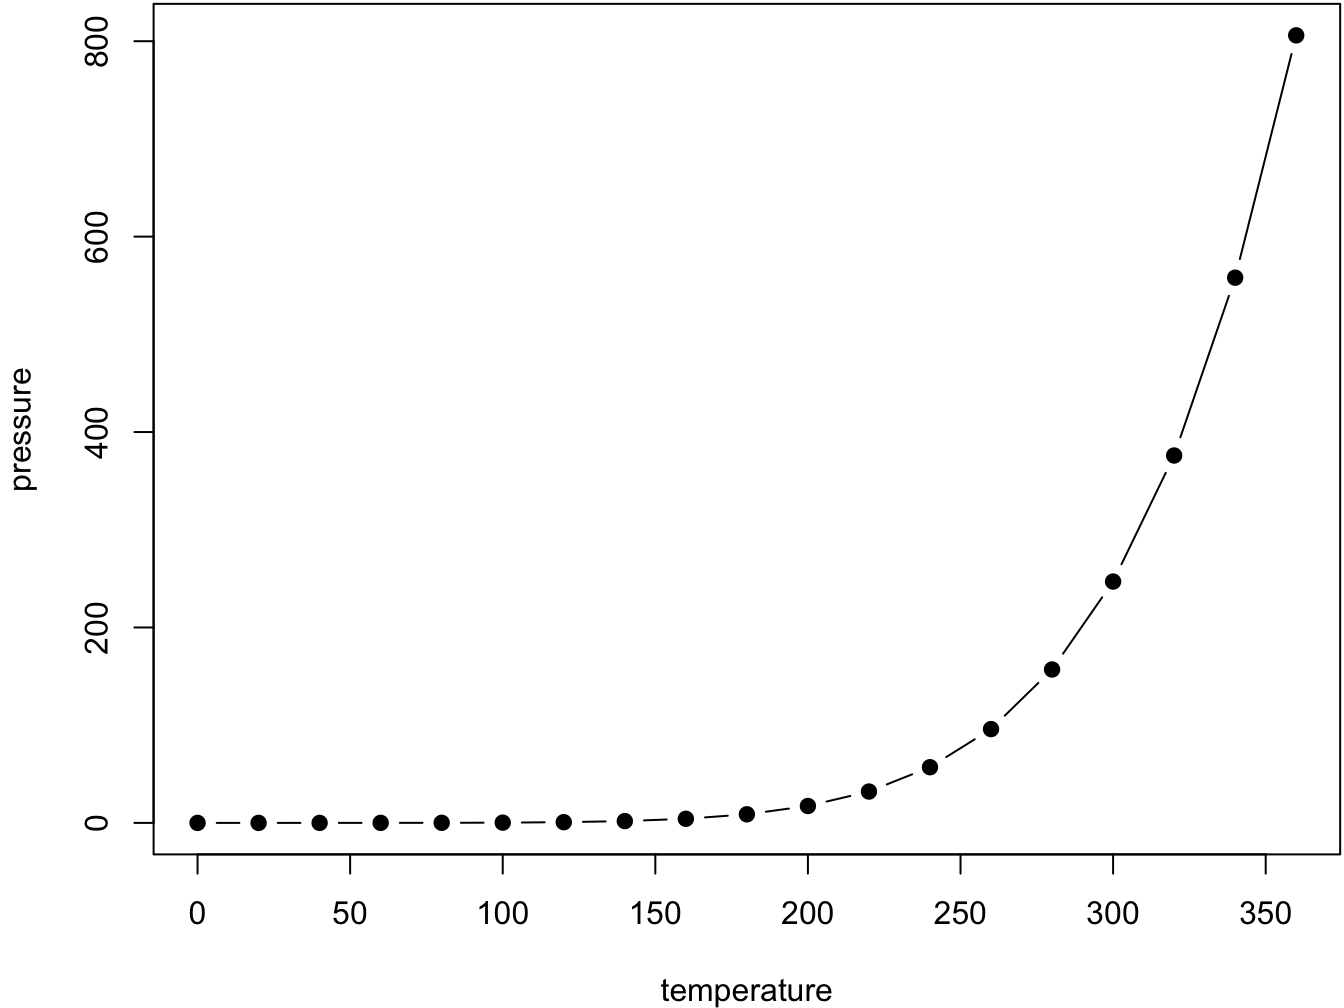
\includegraphics[width=0.8\linewidth]{01-intro_files/figure-latex/nice-fig-1} 

}

\caption{Here is a nice figure!}\label{fig:nice-fig}
\end{figure}

Reference a figure by its code chunk label with the \texttt{fig:} prefix, e.g., see Figure \ref{fig:nice-fig}. Similarly, you can reference tables generated from \texttt{knitr::kable()}, e.g., see Table \ref{tab:nice-tab}.

\begin{Shaded}
\begin{Highlighting}[]
\NormalTok{knitr}\OperatorTok{::}\KeywordTok{kable}\NormalTok{(}
  \KeywordTok{head}\NormalTok{(iris, }\DecValTok{20}\NormalTok{), }\DataTypeTok{caption =} \StringTok{'Here is a nice table!'}\NormalTok{,}
  \DataTypeTok{booktabs =} \OtherTok{TRUE}
\NormalTok{)}
\end{Highlighting}
\end{Shaded}

\begin{table}[t]

\caption{\label{tab:nice-tab}Here is a nice table!}
\centering
\begin{tabular}{rrrrl}
\toprule
Sepal.Length & Sepal.Width & Petal.Length & Petal.Width & Species\\
\midrule
5.1 & 3.5 & 1.4 & 0.2 & setosa\\
4.9 & 3.0 & 1.4 & 0.2 & setosa\\
4.7 & 3.2 & 1.3 & 0.2 & setosa\\
4.6 & 3.1 & 1.5 & 0.2 & setosa\\
5.0 & 3.6 & 1.4 & 0.2 & setosa\\
\addlinespace
5.4 & 3.9 & 1.7 & 0.4 & setosa\\
4.6 & 3.4 & 1.4 & 0.3 & setosa\\
5.0 & 3.4 & 1.5 & 0.2 & setosa\\
4.4 & 2.9 & 1.4 & 0.2 & setosa\\
4.9 & 3.1 & 1.5 & 0.1 & setosa\\
\addlinespace
5.4 & 3.7 & 1.5 & 0.2 & setosa\\
4.8 & 3.4 & 1.6 & 0.2 & setosa\\
4.8 & 3.0 & 1.4 & 0.1 & setosa\\
4.3 & 3.0 & 1.1 & 0.1 & setosa\\
5.8 & 4.0 & 1.2 & 0.2 & setosa\\
\addlinespace
5.7 & 4.4 & 1.5 & 0.4 & setosa\\
5.4 & 3.9 & 1.3 & 0.4 & setosa\\
5.1 & 3.5 & 1.4 & 0.3 & setosa\\
5.7 & 3.8 & 1.7 & 0.3 & setosa\\
5.1 & 3.8 & 1.5 & 0.3 & setosa\\
\bottomrule
\end{tabular}
\end{table}

You can write citations, too. For example, we are using the \textbf{bookdown} package \citep{R-bookdown} in this sample book, which was built on top of R Markdown and \textbf{knitr} \citep{xie2015}.

\hypertarget{clustering-and-differential-expression-workflow}{%
\chapter{Clustering and Differential Expression Workflow}\label{clustering-and-differential-expression-workflow}}

\emph{Author}: Robert A. Amezquita, Fred Hutchinson Cancer Research Center

\hypertarget{introduction}{%
\section{Introduction}\label{introduction}}

Introduce the main purpose of this vignette in paragraph form, why these steps are important, what the end products allow for.

\hypertarget{learning-objectives}{%
\section{Learning objectives}\label{learning-objectives}}

\begin{itemize}
\tightlist
\item
  In bullet form, illustrate what the main outputs are of this vignette
\item
  A couple of bullet points are fine
\end{itemize}

\hypertarget{package-requirements}{%
\section{Package requirements}\label{package-requirements}}

Packages that are required to go through the vignette and how to install them, should largely be through BiocManager interface.

\begin{Shaded}
\begin{Highlighting}[]
\NormalTok{BiocManager}\OperatorTok{::}\KeywordTok{install}\NormalTok{(}\KeywordTok{c}\NormalTok{(}\StringTok{'SC3'}\NormalTok{, }\StringTok{'clusterExperiment'}\NormalTok{, }\StringTok{'BiocParallel'}\NormalTok{, }\StringTok{'BEARscc'}\NormalTok{, }\StringTok{'zinbwave'}\NormalTok{, }\StringTok{'edgeR'}\NormalTok{, }\StringTok{'DESeq2'}\NormalTok{, }\StringTok{'MAST'}\NormalTok{, }\StringTok{'scDD'}\NormalTok{))}
\end{Highlighting}
\end{Shaded}

\hypertarget{loading-the-data}{%
\section{Loading the data}\label{loading-the-data}}

Here the data should be loaded if in package form and briefly explored to illustrate the contents of the data.

If data comes from ``raw'' form, then a simple pipeline for creating the processed data should be illustrated as succinctly as possible.

\begin{Shaded}
\begin{Highlighting}[]
\KeywordTok{library}\NormalTok{(TENxPBMCData)}
\end{Highlighting}
\end{Shaded}

\begin{verbatim}
## Loading required package: SingleCellExperiment
\end{verbatim}

\begin{verbatim}
## Loading required package: SummarizedExperiment
\end{verbatim}

\begin{verbatim}
## Loading required package: GenomicRanges
\end{verbatim}

\begin{verbatim}
## Loading required package: stats4
\end{verbatim}

\begin{verbatim}
## Loading required package: BiocGenerics
\end{verbatim}

\begin{verbatim}
## Loading required package: parallel
\end{verbatim}

\begin{verbatim}
## 
## Attaching package: 'BiocGenerics'
\end{verbatim}

\begin{verbatim}
## The following objects are masked from 'package:parallel':
## 
##     clusterApply, clusterApplyLB, clusterCall, clusterEvalQ,
##     clusterExport, clusterMap, parApply, parCapply, parLapply,
##     parLapplyLB, parRapply, parSapply, parSapplyLB
\end{verbatim}

\begin{verbatim}
## The following objects are masked from 'package:stats':
## 
##     IQR, mad, sd, var, xtabs
\end{verbatim}

\begin{verbatim}
## The following objects are masked from 'package:base':
## 
##     anyDuplicated, append, as.data.frame, basename, cbind,
##     colMeans, colnames, colSums, dirname, do.call, duplicated,
##     eval, evalq, Filter, Find, get, grep, grepl, intersect,
##     is.unsorted, lapply, Map, mapply, match, mget, order, paste,
##     pmax, pmax.int, pmin, pmin.int, Position, rank, rbind, Reduce,
##     rowMeans, rownames, rowSums, sapply, setdiff, sort, table,
##     tapply, union, unique, unsplit, which, which.max, which.min
\end{verbatim}

\begin{verbatim}
## Loading required package: S4Vectors
\end{verbatim}

\begin{verbatim}
## 
## Attaching package: 'S4Vectors'
\end{verbatim}

\begin{verbatim}
## The following object is masked from 'package:base':
## 
##     expand.grid
\end{verbatim}

\begin{verbatim}
## Loading required package: IRanges
\end{verbatim}

\begin{verbatim}
## Loading required package: GenomeInfoDb
\end{verbatim}

\begin{verbatim}
## Loading required package: Biobase
\end{verbatim}

\begin{verbatim}
## Welcome to Bioconductor
## 
##     Vignettes contain introductory material; view with
##     'browseVignettes()'. To cite Bioconductor, see
##     'citation("Biobase")', and for packages 'citation("pkgname")'.
\end{verbatim}

\begin{verbatim}
## Loading required package: DelayedArray
\end{verbatim}

\begin{verbatim}
## Loading required package: matrixStats
\end{verbatim}

\begin{verbatim}
## 
## Attaching package: 'matrixStats'
\end{verbatim}

\begin{verbatim}
## The following objects are masked from 'package:Biobase':
## 
##     anyMissing, rowMedians
\end{verbatim}

\begin{verbatim}
## Loading required package: BiocParallel
\end{verbatim}

\begin{verbatim}
## 
## Attaching package: 'DelayedArray'
\end{verbatim}

\begin{verbatim}
## The following objects are masked from 'package:matrixStats':
## 
##     colMaxs, colMins, colRanges, rowMaxs, rowMins, rowRanges
\end{verbatim}

\begin{verbatim}
## The following objects are masked from 'package:base':
## 
##     aperm, apply
\end{verbatim}

\begin{verbatim}
## Loading required package: HDF5Array
\end{verbatim}

\begin{verbatim}
## Loading required package: rhdf5
\end{verbatim}

\begin{Shaded}
\begin{Highlighting}[]
\KeywordTok{TENxPBMCData}\NormalTok{(}\StringTok{'pbmc4k'}\NormalTok{)}
\end{Highlighting}
\end{Shaded}

\begin{verbatim}
## snapshotDate(): 2019-01-04
\end{verbatim}

\begin{verbatim}
## see ?TENxPBMCData and browseVignettes('TENxPBMCData') for documentation
\end{verbatim}

\begin{verbatim}
## downloading 0 resources
\end{verbatim}

\begin{verbatim}
## loading from cache 
##     '/Users/ramezqui//.ExperimentHub/1613'
\end{verbatim}

\begin{verbatim}
## class: SingleCellExperiment 
## dim: 33694 4340 
## metadata(0):
## assays(1): counts
## rownames(33694): ENSG00000243485 ENSG00000237613 ...
##   ENSG00000277475 ENSG00000268674
## rowData names(3): ENSEMBL_ID Symbol_TENx Symbol
## colnames: NULL
## colData names(11): Sample Barcode ... Individual Date_published
## reducedDimNames(0):
## spikeNames(0):
\end{verbatim}

\hypertarget{preprocessing}{%
\section{Preprocessing}\label{preprocessing}}

All steps required to preprocess the data into the clean expression matrix, split it up into subsections as necessary. Subsection splits should be informed by the paper (sub)sections. This is all steps prior to the main strategy of interest.

\hypertarget{cell-and-gene-quality-control}{%
\subsection{Cell and gene quality control}\label{cell-and-gene-quality-control}}

Removal of ``bad cells'', low abundance genes.

\hypertarget{normalization}{%
\subsection{Normalization}\label{normalization}}

Application of normalization approach, even if its just a log normalization on the count data. Cell cycle normalization may be applicable here.

\hypertarget{feature-selection}{%
\subsection{Feature selection}\label{feature-selection}}

Identifying the subset of the clean matrix to work with.

\hypertarget{dimensionality-reduction}{%
\subsection{Dimensionality reduction}\label{dimensionality-reduction}}

Calculating PCs and UMAP/tSNE representation.

\hypertarget{clustering}{%
\section{Clustering}\label{clustering}}

Strategy 1 of interest. Use BiocParallel. May need to save intermediate data within package to facilitate fast construction of Rmd.

\begin{itemize}
\tightlist
\item
  SC3
\item
  clusterExperiment
\item
  clustree
\item
  BEARscc \# uses ERCC spike ins
\item
  BiocNeighbors \# more for devs
\end{itemize}

\hypertarget{differential-expression}{%
\section{Differential Expression}\label{differential-expression}}

Strategy 2 of interest. Differential expression approaches. Use one of the outputs from above to perform differential expression analyses comparison.

\begin{itemize}
\tightlist
\item
  zinbwave + edgeR/DESeq2 (may exclude as workflow is very different or highlight as an ``advanced section'')
\item
  MAST
\item
  scDD
\item
  SC3
\end{itemize}

\hypertarget{session-info}{%
\section{Session Info}\label{session-info}}

\hypertarget{trajectory-analysis-workflow}{%
\chapter{Trajectory Analysis Workflow}\label{trajectory-analysis-workflow}}

\emph{Author}: Robert A. Amezquita, Fred Hutchinson Cancer Research Center

\hypertarget{introduction-1}{%
\section{Introduction}\label{introduction-1}}

Introduce the main purpose of this vignette in paragraph form, why these steps are important, what the end products allow for.

\hypertarget{learning-objectives-1}{%
\section{Learning objectives}\label{learning-objectives-1}}

\begin{itemize}
\tightlist
\item
  In bullet form, illustrate what the main outputs are of this vignette
\item
  A couple of bullet points are fine
\end{itemize}

\hypertarget{package-requirements-1}{%
\section{Package requirements}\label{package-requirements-1}}

Packages that are required to go through the vignette and how to install them, should largely be through BiocManager interface.

\begin{Shaded}
\begin{Highlighting}[]
\NormalTok{BiocManager}\OperatorTok{::}\KeywordTok{install}\NormalTok{(}\KeywordTok{c}\NormalTok{(}\StringTok{'SC3'}\NormalTok{, }\StringTok{'clusterExperiment'}\NormalTok{, }\StringTok{'BiocParallel'}\NormalTok{, }\StringTok{'BEARscc'}\NormalTok{, }\StringTok{'zinbwave'}\NormalTok{, }\StringTok{'edgeR'}\NormalTok{, }\StringTok{'DESeq2'}\NormalTok{, }\StringTok{'MAST'}\NormalTok{, }\StringTok{'scDD'}\NormalTok{))}
\end{Highlighting}
\end{Shaded}

\hypertarget{loading-the-data-1}{%
\section{Loading the data}\label{loading-the-data-1}}

Here the data should be loaded if in package form and briefly explored to illustrate the contents of the data.

If data comes from ``raw'' form, then a simple pipeline for creating the processed data should be illustrated as succinctly as possible.

\begin{Shaded}
\begin{Highlighting}[]
\KeywordTok{library}\NormalTok{(TENxPBMCData)}
\end{Highlighting}
\end{Shaded}

\begin{verbatim}
## Loading required package: SingleCellExperiment
\end{verbatim}

\begin{verbatim}
## Loading required package: SummarizedExperiment
\end{verbatim}

\begin{verbatim}
## Loading required package: GenomicRanges
\end{verbatim}

\begin{verbatim}
## Loading required package: stats4
\end{verbatim}

\begin{verbatim}
## Loading required package: BiocGenerics
\end{verbatim}

\begin{verbatim}
## Loading required package: parallel
\end{verbatim}

\begin{verbatim}
## 
## Attaching package: 'BiocGenerics'
\end{verbatim}

\begin{verbatim}
## The following objects are masked from 'package:parallel':
## 
##     clusterApply, clusterApplyLB, clusterCall, clusterEvalQ,
##     clusterExport, clusterMap, parApply, parCapply, parLapply,
##     parLapplyLB, parRapply, parSapply, parSapplyLB
\end{verbatim}

\begin{verbatim}
## The following objects are masked from 'package:stats':
## 
##     IQR, mad, sd, var, xtabs
\end{verbatim}

\begin{verbatim}
## The following objects are masked from 'package:base':
## 
##     anyDuplicated, append, as.data.frame, basename, cbind,
##     colMeans, colnames, colSums, dirname, do.call, duplicated,
##     eval, evalq, Filter, Find, get, grep, grepl, intersect,
##     is.unsorted, lapply, Map, mapply, match, mget, order, paste,
##     pmax, pmax.int, pmin, pmin.int, Position, rank, rbind, Reduce,
##     rowMeans, rownames, rowSums, sapply, setdiff, sort, table,
##     tapply, union, unique, unsplit, which, which.max, which.min
\end{verbatim}

\begin{verbatim}
## Loading required package: S4Vectors
\end{verbatim}

\begin{verbatim}
## 
## Attaching package: 'S4Vectors'
\end{verbatim}

\begin{verbatim}
## The following object is masked from 'package:base':
## 
##     expand.grid
\end{verbatim}

\begin{verbatim}
## Loading required package: IRanges
\end{verbatim}

\begin{verbatim}
## Loading required package: GenomeInfoDb
\end{verbatim}

\begin{verbatim}
## Loading required package: Biobase
\end{verbatim}

\begin{verbatim}
## Welcome to Bioconductor
## 
##     Vignettes contain introductory material; view with
##     'browseVignettes()'. To cite Bioconductor, see
##     'citation("Biobase")', and for packages 'citation("pkgname")'.
\end{verbatim}

\begin{verbatim}
## Loading required package: DelayedArray
\end{verbatim}

\begin{verbatim}
## Loading required package: matrixStats
\end{verbatim}

\begin{verbatim}
## 
## Attaching package: 'matrixStats'
\end{verbatim}

\begin{verbatim}
## The following objects are masked from 'package:Biobase':
## 
##     anyMissing, rowMedians
\end{verbatim}

\begin{verbatim}
## Loading required package: BiocParallel
\end{verbatim}

\begin{verbatim}
## 
## Attaching package: 'DelayedArray'
\end{verbatim}

\begin{verbatim}
## The following objects are masked from 'package:matrixStats':
## 
##     colMaxs, colMins, colRanges, rowMaxs, rowMins, rowRanges
\end{verbatim}

\begin{verbatim}
## The following objects are masked from 'package:base':
## 
##     aperm, apply
\end{verbatim}

\begin{verbatim}
## Loading required package: HDF5Array
\end{verbatim}

\begin{verbatim}
## Loading required package: rhdf5
\end{verbatim}

\begin{Shaded}
\begin{Highlighting}[]
\KeywordTok{TENxPBMCData}\NormalTok{(}\StringTok{'pbmc4k'}\NormalTok{)}
\end{Highlighting}
\end{Shaded}

\begin{verbatim}
## snapshotDate(): 2019-01-04
\end{verbatim}

\begin{verbatim}
## see ?TENxPBMCData and browseVignettes('TENxPBMCData') for documentation
\end{verbatim}

\begin{verbatim}
## downloading 0 resources
\end{verbatim}

\begin{verbatim}
## loading from cache 
##     '/Users/ramezqui//.ExperimentHub/1613'
\end{verbatim}

\begin{verbatim}
## class: SingleCellExperiment 
## dim: 33694 4340 
## metadata(0):
## assays(1): counts
## rownames(33694): ENSG00000243485 ENSG00000237613 ...
##   ENSG00000277475 ENSG00000268674
## rowData names(3): ENSEMBL_ID Symbol_TENx Symbol
## colnames: NULL
## colData names(11): Sample Barcode ... Individual Date_published
## reducedDimNames(0):
## spikeNames(0):
\end{verbatim}

\hypertarget{preprocessing-1}{%
\section{Preprocessing}\label{preprocessing-1}}

All steps required to preprocess the data into the clean expression matrix, split it up into subsections as necessary. Subsection splits should be informed by the paper (sub)sections. This is all steps prior to the main strategy of interest.

\hypertarget{cell-and-gene-quality-control-1}{%
\subsection{Cell and gene quality control}\label{cell-and-gene-quality-control-1}}

Removal of ``bad cells'', low abundance genes.

\hypertarget{normalization-1}{%
\subsection{Normalization}\label{normalization-1}}

Application of normalization approach, even if its just a log normalization on the count data. Cell cycle normalization may be applicable here.

\hypertarget{feature-selection-1}{%
\subsection{Feature selection}\label{feature-selection-1}}

Identifying the subset of the clean matrix to work with.

\hypertarget{dimensionality-reduction-1}{%
\subsection{Dimensionality reduction}\label{dimensionality-reduction-1}}

Calculating PCs and UMAP/tSNE representation. This may not be necessary for certain software or may differ between packages.

\hypertarget{trajectory-analysis}{%
\section{Trajectory Analysis}\label{trajectory-analysis}}

\begin{itemize}
\tightlist
\item
  slingshot
\item
  ouija
\item
  celltrails
\end{itemize}

\hypertarget{session-info-1}{%
\section{Session Info}\label{session-info-1}}

\bibliography{book.bib,packages.bib}


\end{document}
